\documentclass[12pt,-letter paper]{article}
\usepackage{gvv}
\begin{document}
\begin{enumerate}
\item the boolen function realized by the logic circuit shown is
\begin{figure}[H]
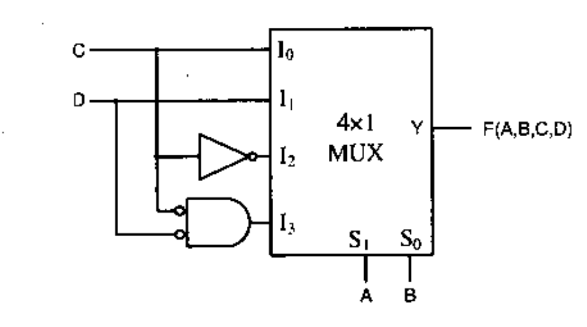
\includegraphics[width=\columnwidth]{./gate1.png}
\label{fig:fig1}
\caption{}
\end{figure}

\begin{enumerate}
	\item $F=\sum_m\brak{0,1,3,5,9,10,14}$
	\item $F=\sum_m\brak{2,3,5,7,8,12,13}$
	\item $F=\sum_m\brak{1,2,4,5,11,14,15}$
	\item $F=\sum_m\brak{2,3,5,7,8,9,12}$	
\end{enumerate}

\end{enumerate}
\end{document}

